\begin{frame}
  \frametitle{Maximum-Likelihood Estimation}
  \begin{center}
    Maximum-likelihood estimation (MLE) is a method for estimating the parameters
    of a probability model from a set of observations.
    \vspace{3em}
    
    MLE chooses the parameters that make the observations most probable.
  \end{center}
\end{frame}

\begin{frame}
  \frametitle{What are the parameters of the Gaussian distribution over kitten
    paw width?}
  \begin{center}
    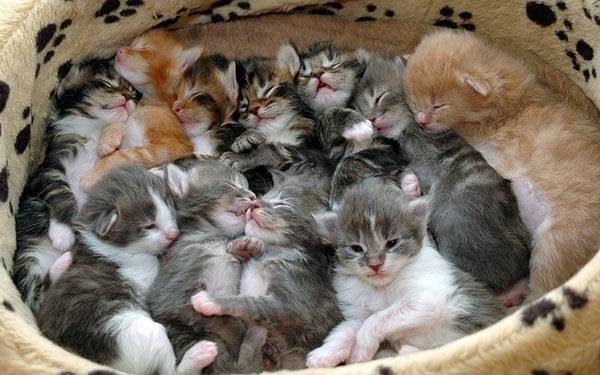
\includegraphics[width=3.7in]{img/Kittens.jpg}

    Because cute kittens immediately make you think of Gaussian distributions.
  \end{center}
\end{frame}

\begin{frame}
  \frametitle{Kitten paw width likelihood model}
  Paw width is Gaussian distributed with mean $\mu^*$ and variance ${\sigma^*}^2$.
  \vspace{1em}

  We have $n$ observations $w_1, w_2, ..., w_n$
  \vspace{1em}

  Likelihood of a given observation $w_i$:
  \[p(w_i|\mu, \sigma) = \frac1{ \sigma \sqrt{2 \pi}} \exp{\left[ \frac{(w_i -
      \mu)^2}{2 \sigma^2} \right]}\]

  Observations are independent:
  \[p(w_1, w_2, \ldots, w_n|\mu, \sigma) = \displaystyle \prod_{i=1}^n p(w_i|\mu, \sigma)\]

\end{frame}

\begin{frame}
\frametitle{Calculating the kitten paw width parameters}
  Find $\mu^*$ and $\sigma^*$ by maximizing:
  \[\mu^*, \sigma^* = \argmax_{\mu, \sigma}{p(w_1, w_2, \ldots, w_n|\mu,
    \sigma)} = \argmax_{\mu, \sigma}{\displaystyle \prod_{i=1}^n p(w_i|\mu,
    \sigma)}\]

  Because $\log$ is a monotonically increasing function, we can convert this
  into the more computationally attractive:
  \[\mu^*, \sigma^* = \argmax_{\mu, \sigma}{\log{p(w_1, w_2, \ldots, w_n|\mu,
    \sigma)}} = \argmax_{\mu, \sigma}{\displaystyle \sum_{i=1}^n \log{p(w_i|\mu,
    \sigma)}}\]
\end{frame}